

The system used to generate and process aerosols is illustrated in Figure \ref{fig:system}. It comprised an aerosol generation unit (either an atomizer or an inverted diffusion flame burner), a differential mobility analyzer (DMA, TSI Model 3081A) with home-built recirculating sheath flow and high voltage control to produce electrical mobility-classified aerosol, a temperature-controlled coating chamber, a thermal denuder to remove coating from aerosol \citep{RN39}, an aerosol particle mass analyzer (APM, Kanomax Model 3601) to measure mass of aerosol particles, a second DMA to measure electrical mobility diameter of aerosol particles processed by coating or coating followed by denuding, a cavity attenuated phase shift spectrometer (CAPS PM\textsubscript{SSA}, Aerodyne Research, 525 nm wavelength) to measure aerosol extinction and scattering coefficients, and a condensation particle counter (CPC, TSI Model 3772) to measure aerosol particle number density. The components of the system were connected with stainless steel tubing segments joined together with conductive silicone tubing. The entire system was conrolled by LabView codes, and a detailed description of the system and its individual components can be found in our previous work \citep{RN48,RN49}.

\begin{figure}[ht]
\centering
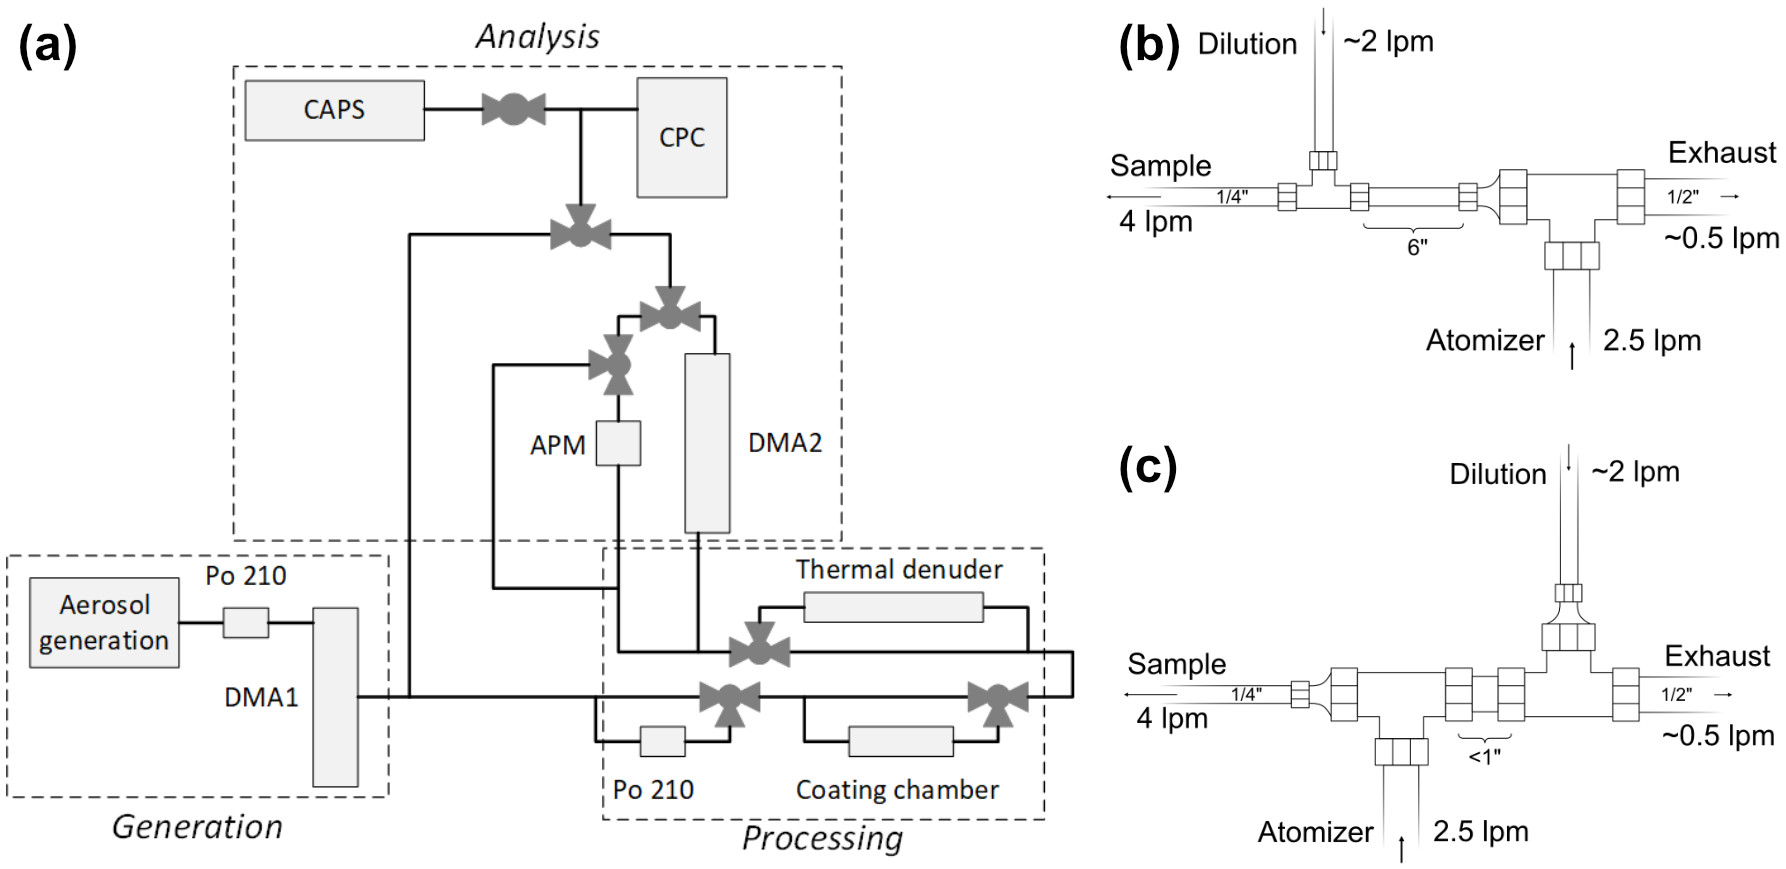
\includegraphics[width=\textwidth]{system_diagram.png}
\caption{Aerosol generation and processing system}
\label{fig:system}
\end{figure}

\subsection{Particle generation and processing}

Soot was generated by incomplete combustion of natural gas in an inverted diffusion flame burner \citep{RN43,RN44} and sampled using an ejector dilutor. Carbon black suspension (Cab-O-Jet 200, Cabot Corporation) and nigrosin solution (Nigrosin water soluble, Alfa Aesar) were prepared with distilled water and corresponding aerosols were generated with a constant output atomizer (TSI Model 3076). To generate compact CB, the nebulized aqueous aerosol was immediately diluted with dry air. To generate agglomerated CB, the nebulized aerosol was diluted a few centimeters downstream from the atomizer, which provided sufficient residence time for concentrated aerosol droplets to coagulate, producing agglomerated CB particles after drying. In some experiments, polystyrene latex (PSL) aerosols of different particle sizes were generated from suspensions of nanospheres (3000 Series Nanosphere, Thermo Scientific). The aerosols were brought to quilibrium charge distribution with a bipolar \textsuperscript{210}Po charger (Staticmaster Static Eliminator, 500 µCi) and size-classified with DMA1. It is important to note that particles carrying multiple charges behave as if they were smaller in an electric field of the DMA. Therefore, aerosol after DMA1 is pseudo-monodisperse.

The size-classified aerosol was coated by passing it through a temperature-controlled coating chamber, which is a cylindrical borosilicate glass container (45 cm length and 2 cm inner diameter) partially filled with dioctyl sebacate and wrapped in heating tape and insulation. DOS was selected as the coating material because of its low volatility (saturated vapor pressure of $9.69\times10^{-6}\ \mathrm{Pa}$ at $25\ \mathrm{^{\circ}C}$) and frequent use to study soot processing and optics.
%\textcolor{red}{Do we need the following sentence here? [The refractive index of DOS (1.43+0i) is in the range of refractive indices of many liquid coating materials \citep{RN22}]}.
Adjusting the temperature of the coating chamber allowed the control of DOS condensation on particles. In some experiments, the condensed coating material was subsequently removed from particles by passing them through a thermal denuder operated at 300 °C. All particles were passed through an identical denuder prior to aging to ensure that any optical response of coated-denuded particles was not induced by the high temperature in the denuder. Particle mass and electrical mobility diameter of processed aerosol were measured by sending the flow through the APM and DMA2, respectively. Both DMAs were operated at a sheath-to-sample flow ratio of 6.5, using sample and sheath flows of 1.0 and 6.5 liters per minute (lpm). The APM operated at a sample flow of 0.3 lpm, which was achieved by removing 0.7 lpm before the APM and then adding 0.7 lpm of filtered clean air after the APM, using volumetric flow controllers connected to a vacuum pump and pressurized air, respectively.

Mass measurements were used to determine the amount of coating condensed and electrical mobility diameter was used to quantify the extent of restructuring. Mass of processed particles, $m$ was normalized by mass of fresh particles $m_0$ to obtain the mass growth factor.
\begin{equation}
\mathrm{Gfm}=\frac{m}{m_0}
\label{eq:gfm}
\end{equation}
Mass growth factor was converted into volume-equivalent coating thickness, $\Delta r_{ve}$, to facilitate the comparison in the amount of coating gained by particles of different initial volume-equivalent diameters \citep{RN37}.
\begin{equation}
\Delta r_{ve}=\frac{1}{2}D_{ve,0}\left(\sqrt[3]{\frac{V}{V_0}}-1\right)=
\frac{1}{2}D_{ve,0}\left(\sqrt[3]{1+\frac{\rho_{\rm core}}{\rho_{\rm shell}}\left(\mathrm{Gfm}-1\right)}-1\right)
\label{eq:drve}
\end{equation}
Where $D_{\rm ve,0}$ is volume-equivalent diameter of a bare particles, $V$ is volume of a coated particle, $V_0$ is volume of a bare particle, $\rho_{\rm core}$ is material density of a bare particle, and $\rho_{\rm shell}$ is density of the coating material.

Similarly, the electrical mobility diameter of processed particles, $D$ was normalized by the electrical mobility diameter of fresh particles, $D_0$, to obtain the electrical mobility diameter growth factor.
\begin{equation}
\mathrm{Gfd}=\frac{D}{D_0}
\label{eq:gfd}
\end{equation}
$GF_{\rm d}$ was obtained from Tandem DMA (TDMA) scans, where particles were size-classified with DMA1, processed by coating or coating-denuding, and then their size distribution was measured with DMA2.

\subsection{Particle sample collection and imaging}

Samples of size-classified unprocessed aerosol particles were collected on silicon chips, using a custom-built electrostatic precipitator \citep{RN17,RN16} placed after DMA1. In the precipitator, high voltage (3-4 kV) applied to the chip holder created an electric field between the chip and grounded body of the precipitator, causing charged aerosol particles to travel toward and deposit on the silicon chip. After an hour of collection, chips were removed from the precipitator and imaged with a scanning electron microscope (SEM, JEOL JSM-7900F). Before collection, silicon chips were prepared by washing with methanol in an ultrasound bath and drying with nitrogen gas. To quantify particle compactness, convexity was calculated from SEM images as the ratio of the particle projected area ($A_p$) to the area of a convex hull polygon.

\begin{equation}
    \mathrm{Convexity}=\frac{A_p}{A_{polygon}}
    \label{eq:convexity}
\end{equation}

\subsection{Optical measurements}

To measure number density and optical properties of aerosol concurrently, a makeup flow of 0.87 lpm was added and then the sample flow was split iso-kinetically in two separate flows directed to CAPS PM\textsubscript{SSA} (0.87 lpm) and CPC (1.0 lpm), respectively. An orifice inside the valve ensured mixing of the aerosol stream and the dilution air stream. The distances from the split to CAPS PM\textsubscript{SSA} and CPC were adjusted to ensure equal wall losses, so that the particle number density measured by the CPC corresponded to the number density within the CAPS PM\textsubscript{SSA} cell. We found that it was crucial to install a denuder filled with XB-17 (a mixture of activated charcoal and permanganate-impregnated alumina, General Carbon Corp.) after DMA1 during experiments with flame-generated soot to remove traces of NO\textsubscript{2} produced by the burner. NO\textsubscript{2} is a strong light absorber at 525 nm and its concentration is highly sensitive to combustion conditions. In the absence of the denuder, light extinction measurements were subject to significant variability, requiring that baselines to be taken frequently.

The CAPS PM\textsubscript{SSA} measured extinction and scattering coefficients ($b$) of bare and processed aerosol particles. Absorption coefficients were calculated as a difference of extinction and scattering coefficients \citep{RN7,RN50}.
\begin{equation}
b_{\rm abs}=b_{\rm ext}-b_{\rm sca}
\label{eq:babs}
\end{equation}
The coefficients were converted to cross sections ($C$) by normalizing them by aerosol number density ($N$):
\begin{equation}
C=\frac{b}{N}
\label{eq:copt}
\end{equation}

To obtain accurate optical data, scattering and extinction coefficients were recorded every five seconds over three minutes for each measurement. Arithmetic mean of the cross sections acquired over a three-minute interval was calculated and reported as the optical measurement. Baselines were taken prior to each measurement, where aerosol flow was redirected through a filter (United Filtration DIF-BN60) located inside the CAPS PM\textsubscript{SSA} to flush its optics cell and measure extinction and scattering of gas without particles.

\subsection{Numerical aggregate generation for discrete dipole approximation calculations}

Soot aggregates of fractal ($D_f < 2.1$) and compact ($D_f > 2.1$) morphologies were simulated using a cluster-cluster aggregation (CCA) algorithm developed by \citet{RN35}. The CCA method, described here in brief, is based on a hierarchical scheme of aggregation of smaller sub-clusters, which obey the fractal scaling law \citep{jullien1987aggregation},
\begin{equation}
N_s=k_0\left(\frac{2R_s}{d_p}\right)^{D_f}
\label{eq:fractal}
\end{equation}
where $N_s$ is the number of primary particles, $k_0$ is the pre-exponential factor, $R_s$ is the radius of gyration, $d_p$ is the diameter of primary units, and $D_f$ is the fractal dimension. In this context, where all the primary particles are assumed to be of the same size, $R_g$ is defined as the root mean squared distance of primary particles from the center of mass of the aggregate. Equal-sized primary particles are characteristic of many laboratory generated soot aggregates \citep{RN22,RN25}.

Aggregate generation involves sequentially combining smaller sub-aggregates into bigger clusters until the target aggregate size $N$ is reached. Every time two sub-aggregates are combined into a cluster, radius of gyration of the formed cluster, $R_{g,\rm new}$, depends on radii of gyration of its two constituent sub-aggregates, $R_{g,1}$ and $R_{g,2}$, and on how those sub-aggregates are combined. Therefore, $R_{g,\rm new}$ of the formed cluster can be controlled by varying the orientations of the sub-aggregates and the location of the point where they are joined. A function $R_{g,\rm new}(R_{g,1},R_{g,2},D_f,k_0)$ is derived from the fractal scaling law and the definition of $R_g$. Then, at every step where sub-aggregates are combined, $R_{g,\rm new}$ is prescribed by the fractal scaling law and orientations and joining positions are varied randomly until $R_{g,\rm new}$ of the combined cluster is within error tolerance from the target value. Thus, by constraining the way sub-aggregates are combined, an aggregate conforming to Equation \ref{eq:fractal} is generated. Aggregates produced by the CCA algorithm are representative of real soot particles formed via diffusion-limited cluster aggregation \citep{RN36}.

To discretize the aggregate for use with DDA, a three-dimensional Cartesian grid is created and the generated fractal aggregate is placed in this Cartesian space. For each spherical particle comprising the aggregate, grid elements that fall within the boundary of the sphere are filled with black carbon. To add a uniform coating to the discretized aggregate, the function described in \citet{RN22} is used to compute the boundary of the coating layer and all the grid elements that are within the boundary of the coating, but are not already filled with black carbon, are then filled with the coating material.

% The aggregate generation process begins with a set of isolated identical spherical primary particles, $N_M \ge N_s$. A random pair is picked and joined at a random contact point leaving $N_M–1$ primary particles. A new pair is selected from the set and joined. The combination of a pair of clusters is constrained by the distance between the centers of masses of the two clusters, which is such that Equation \eqref{eq:fractal} still holds. The combining clusters are then rotated as solid bodies until they have at least one contact point and no overlapping. After performing the procedure for all clusters on one level, another level involving larger clusters begins and the procedure is repeated till the aggregate attains the desired number of primary particles, $N_s$, which was set to 120, roughly corresponding to fractal soot aggregates of 240 nm mobility diameter used in our experiments. The simulated aggregates are assumed to be monodisperse with a primary particle diameter, $R_s$ set to 28 nm, which is typical for some laboratory generated soot aggregates \citep{RN22,RN25}. To generate coated soot, the coating material was applied to obtain a uniform coating distribution on the bare aggregates as described by \citet{RN22}. Aggregates produced by the CCA algorithms are representative of real soot particles formed via diffusion-limited cluster aggregation \citep{RN36}.

\subsection{Optical models}

Mie theory, Rayleigh-Debye-Gans (RDG),  and discrete dipole approximation (DDA) were used to predict optical properties of bare and coated particles. Mie theory provides a solution for electromagnetic wave scattering and extinction by a sphere \citep{RN1}. A modification of Mie for coated spheres, implemented by \cite{RN19}, was used to model coated particles in this study. Mie provides an exact solution for spherical particles (e.g., nigrosin) and should be in a reasonable agreement with experimental data for compact particles, such CB, thickly coated soot, or coated-denuded soot, due to their near-spherical shape.

The RDG approximation \citep{RN40,kerker2016scattering} can be used to provide a better estimate of optical properties in the case of fractal aggregates. Absorption cross section (Equation \ref{eq:rdg}) of an aggregate is approximated by a product of the absorption cross section of an individual primary particle ($C_\mathrm{abs,monomer}$) and the number of individual primary particles ($N$). In conjunction with core-shell Mie theory, RDG can be used to predict light absorption by thinly coated fractal aggregates (RDG-Mie). We do not consider RDG scattering because it requires the fractal dimension of aggregates, experimental determination of which is beyond the scope of this study. To extend the RDG approach to coated aggregates, the coating material is distributed over the primary particles as spherical shells and absorption cross sections are computed for the coated primary particles using core-shell Mie. Then, absorption cross sections of coated primary particles are scaled to aggregates according to RDG theory.
\begin{equation}
    C_\mathrm{abs,aggregate}=NC_\mathrm{abs,monomer}
    \label{eq:rdg}
\end{equation}
When the diameter of primary particles in an aggregate is known, volume equivalent coating thickness of a primary particle can be related to volume-equivalent coating thickness of the aggregate with Equation \ref{eq:drve_monomer}:
\begin{equation}
    \Delta r_{m}=d_m\frac{\Delta r_{ve}}{D_0}
    \label{eq:drve_monomer}
\end{equation}

DDA \citep{RN33} is a versatile approach for predicting the optical properties of particles of arbitrary geometry that has been used in a large number of soot modeling studies \citep{RN26,RN27,RN28}. In DDA, the particle shape is described as a collection of small discrete volumes (dipoles) that interact with electromagnetic waves and each other. To converge to an accurate solution, the interdipole separation, $d$, has to be chosen sufficiently small such that the quantity $|n|kd < 1$, where $n$ is the complex refractive index and $k = 2\pi/\lambda$ is the wavenumber, with $\lambda$ being the incident wavelength. This is to ensure that the dipole approximation holds \citep{RN29} and that the geometry of the particle is well approximated by an array of dipoles \citep{RN30}.

Optical modeling was performed using the refractive indices shown in Table \ref{tab:refindices}. The refractive index of soot is based on the expression reported by \citet{RN23}. For a wavelength of 530 nm, the refractive index was $1.73+0.6i$, falling within the range recommended by \citet{RN34} for visible light. The refractive index of the organic coating was assumed to be $1.43+0i$ and is representative of many organic materials \citep{crchandbook}, including DOS, which was used in our experiments. By comparing DOS with other chemicals of similar structure, we found that the refractive index varied by less than  $\pm0.03$, causing a $\pm 3.5\%$ variation in scattering and $\pm 2.5\%$ variation in absorption by a 150 nm absorbing sphere with a 20 nm coating. Such variation is within the error range of our experimental measurements.

Optical measurements were conducted at 525 nm wavelength, while DDA calculations were performed for 530 nm wavelength. According to our sensitivity analysis, the difference in scattering is $0.4 \%$ and the difference in absorption is $0.3 \%$ for a 150 nm absorbing sphere with a 20 nm coating at 525 and 530 nm wavelength. This difference is within the error of our experimental measurements, which means that DDA calculations are representative of experimental data.

\begin{table}[ht]
\caption{Refractive indices of materials used in optical calculations}
\label{tab:refindices}
\begin{center}
\begin{tabular}{ l c }
 \hline
 \multicolumn{1}{c}{Material} & Complex refractive index \\
 \hline
 Soot/carbon black\textsuperscript{\textit{a}} & 1.73+0.60i\\
 Nigrosin\textsuperscript{\textit{b}} & 1.71+0.27i\\
 Liquid organic compounds\textsuperscript{\textit{c}} & 1.43+0.00i\\
 \hline
\end{tabular}
\end{center}

\textsuperscript{\textit{a}}\citet{RN23}\\
\textsuperscript{\textit{b}}\citet{RN15}\\
\textsuperscript{\textit{c}}\citet{RN22}
\end{table}

For this study, the Amsterdam DDA (ADDA) version 1.3 \citep{RN11}, an open-source C implementation of DDA, was used. For each bare or coated soot aggregate, orientation-averaged extinction, scattering, and absorption cross-sections ($C_{\rm ext}$, $C_{\rm sca}$, $C_{\rm abs}$) were determined. The interdipole separation, $d$ was varied from 2 nm down to 0.8 nm, resulting in approximately 1400 to 22,000 dipoles per single monomer volume. The maximum dipole size of 2 nm was only used for thickly coated aggregates (i.e., $\Delta r_{ve}\ge 18\ \rm nm$). Small dipole sizes ensured that both the coating and morphological features were accurately represented i.e., there were no shape approximation errors. Under these circumstances $|m|kd$, was less than 0.1 and satisfied the restriction set by \citet{RN32} for obtaining accurate optical predictions for soot aggregates. The calculated optical properties presented in this study are an average of three aggregate realizations belonging to the same class of fractal parameters ($N_s$, $R_s$, $D_f$, $k_0$). The relative standard deviations (RSD) obtained were less than $1\%$.
